% Complete 8-page working manuscript; generated by scripts/build-length-variants.mjs.
% IEEE working format; target-venue compliance requires the conference handoff.
% !TeX program = pdflatex
\RequirePackage[T1]{fontenc}
\documentclass[conference]{IEEEtran}
\IEEEoverridecommandlockouts

\usepackage{amsmath}
\usepackage{booktabs}
\usepackage{cite}
\usepackage{graphicx}
\usepackage[hidelinks]{hyperref}
\usepackage{tikz}
\usepackage{xpatch}
\usetikzlibrary{arrows.meta,positioning,fit}

\renewcommand{\textbullet}{\textnormal{-}}
\renewcommand{\labelitemi}{\textnormal{-}}
\renewcommand{\labelitemii}{\textnormal{-}}
\emergencystretch=2em
\interdisplaylinepenalty=2500
\newcommand{\Description}[1]{}
\xpatchcmd{\abstract}{---}{-}{}{}
\xpatchcmd{\IEEEkeywords}{---}{-}{}{}

\newif\ifarchsyncanonymous
\ifdefined\archsyncanonymousmode
  \archsyncanonymoustrue
\else
  \archsyncanonymousfalse
\fi
\newcommand{\archsyncrepository}[2]{%
  \ifarchsyncanonymous
    \nolinkurl{#1} (blinded)%
  \else
    \href{#2}{\nolinkurl{#1}}%
  \fi
}
\newcommand{\archsynccommit}[4]{%
  \ifarchsyncanonymous
    \texttt{#1} commit \texttt{#4} (blinded artifact)%
  \else
    \href{#2/commit/#3}{\texttt{#1} commit \texttt{#4}}%
  \fi
}

\begin{document}

\title{ArchSync: A Controlled Feasibility Study of Evidence-Backed Architecture Drift Detection in TypeScript Systems}

\ifarchsyncanonymous
  \author{\IEEEauthorblockN{\archsyncanonymousauthor}}
\else
  \author{%
    \IEEEauthorblockN{Vo Duc Hieu\IEEEauthorrefmark{1},
      Tran Minh Hoang\IEEEauthorrefmark{2},
      Ha Hoang Bach\IEEEauthorrefmark{3},
      Le Van Kiet\IEEEauthorrefmark{4},\\
      Hoang Nguyen The\IEEEauthorrefmark{5}, and
      Minh Tam Phan\IEEEauthorrefmark{5}}
    \IEEEauthorblockA{\IEEEauthorrefmark{1}Software Engineering, FPT University, Ho Chi Minh City, Vietnam\\
      Email: voduchieu@littleboys.biz; ORCID: 0009-0007-5389-5177}
    \IEEEauthorblockA{\IEEEauthorrefmark{2}Computer Science and Engineering, VNUK Institute for Research and Executive Education,\\
      The University of Danang, Da Nang, Vietnam\\
      Email: an1dee@littleboys.biz; ORCID: 0009-0000-0302-1841}
    \IEEEauthorblockA{\IEEEauthorrefmark{3}Information Assurance, FPT University, Ho Chi Minh City, Vietnam\\
      Email: bachcp6@littleboys.biz; ORCID: 0009-0000-5118-0660}
    \IEEEauthorblockA{\IEEEauthorrefmark{4}Software Engineering, VNUK Institute for Research and Executive Education,\\
      The University of Danang, Da Nang, Vietnam\\
      Email: levankiet1212.2004@littleboys.biz; ORCID: 0009-0007-8434-882X}
    \IEEEauthorblockA{\IEEEauthorrefmark{5}Faculty of Software Engineering, FPT University HCMC,\\
      Ho Chi Minh City, 70000, Vietnam\\
      Email: hoangnt20@fe.edu.vn, tampm@fe.edu.vn}
    \thanks{Corresponding author: Vo Duc Hieu (voduchieu@littleboys.biz).}
  }
\fi

\maketitle

\begin{abstract}
Software teams can keep builds green while implementation relationships drift away from an approved architecture, leaving reviewers without a repeatable way to decide whether a change is harmless, forbidden, or a legitimate evolution. This paper presents ArchSync, a deterministic architecture-conformance prototype that treats a machine-readable model as an executable contract and reconstructs an observed service graph from TypeScript source code. Stack-specific analyzers detect selected HTTP, PostgreSQL, Redis, and AMQP interactions, preserve file-level evidence, and feed a Git-diff gate that maps introduced findings to PASS, BLOCK, or REVIEW without rewriting the approved model. We verify the prototype on two co-developed development datasets and replay the same controlled changes through the incremental gate. Within these finite regression sets, the implementation agrees with the declared graph, decision, evidence-location, and full-scan oracles, and provenance tracking removes the targeted detector errors exposed by the earlier analyzer. An external-tool comparison remains proposed and was not executed within the reported evaluation; no accepted comparator result or common label mapping is available, and the study lacks an independently curated real-world holdout. Its results therefore establish executable-contract coherence and reproducible regression behavior only, not comparative advantage or general accuracy on TypeScript systems.
\end{abstract}


\begin{IEEEkeywords}
software architecture, architecture conformance, architecture drift, static analysis, architecture as code
\end{IEEEkeywords}

\section{Introduction}
Software architecture defines intended components and permitted relationships. Evolution can introduce structural violations while compilation and functional tests remain green; mapping and practitioner studies describe erosion and continuing reliance on documentation and shared practices \cite{li2022erosion,anthony2024drifting}. A seemingly local change can bypass a gateway, access a database directly, or add infrastructure without an architecture decision.

ArchSync connects a versioned expected graph from \texttt{architecture.yaml} to an observed graph reconstructed from source. Explicit deny, allow, require, and require-path rules distinguish broken constraints from non-forbidden topology changes. Evidence links findings to implementation and model locations. For pull requests, only findings introduced relative to the Git merge base determine PASS, BLOCK, or REVIEW; historical findings remain visible. The observed graph follows code, while the expected graph remains approved intent. REVIEW requests a human decision and does not itself implement approval or rejection governance.

The prototype detects selected TypeScript/Node.js HTTP, PostgreSQL, Redis, and AMQP patterns. The model and conformance contracts are language-neutral, but only this source analyzer has empirical evidence. Determinism makes repeated explicit-rule decisions reproducible; it does not imply complete extraction or general accuracy. AI explanations, automatic repairs, IaC, and runtime observations remain outside the evaluated decision path.

The contributions are: (1) a typed executable-contract prototype with source/model evidence, (2) a relation-level incremental PR gate, and (3) a controlled verification artifact with explicit units and provenance. They are bounded prototype contributions, not new conformance concepts or validated industrial effectiveness.

\section{Background and Related Work}
This scoped narrative synthesis establishes context for ArchSync's design; it is not a systematic literature review. Sources were selected purposively from the retained keyword-search corpus for architecture conformance, drift detection, and static-analysis reliability, emphasizing 2022--2025. Four earlier works supply concept origins. Selection and interpretation may omit relevant approaches; coverage completeness and absence-of-prior-work claims are outside scope.

\textbf{Erosion and reconstruction.} A mapping of architecture erosion describes its manifestations and consequences \cite{li2022erosion}. Code-review studies identify symptoms in OpenStack and later OpenStack/Qt projects \cite{li2022symptoms,li2023warnings}; their shared project contexts are not independent replications. Practitioner evidence identifies documentation, responsibilities, and shared practices as ways to manage drift \cite{anthony2024drifting}. Reconstruction taxonomies organize recovery strategies \cite{ducasse2009reconstruction,sar2024taxonomy}, while a microservice mapping compares tool purposes and availability \cite{bakhtin2024mapping}. View-based analysis compares intended and reconstructed specifications in an industrial case \cite{uzun2024drift}. ArchSync restricts its observation boundary to explicit service and infrastructure relationships.

\textbf{Conformance.} Reflexion Models, static conformance comparisons, and DCL provide the origins of model comparison and allowed/forbidden dependency rules \cite{murphy1995reflexion,knodel2007comparison,terra2009dcl}; neither concept is new here. CALint applies dependency-rule checks to Python \cite{calint2022}. ArchLintor is a close TypeScript comparison, detecting module-interaction violations and supporting CI/CD \cite{archlintor2025}. ArchSync's typed service topology differs from that module boundary; no head-to-head accuracy result is claimed. IaC metrics address deployment coupling \cite{ntentos2022iac}, and 3Erefactor searches for executable inconsistency-reducing repairs \cite{refactor2024}. LLM-generated architectural tests distinguish execution success from correct rule expression \cite{lucena2025gatekeepers}. ArchSync executes explicit rules deterministically, but that choice alone implies neither accuracy nor superiority.

\textbf{Change-time feedback.} Commit-level prediction studies architectural change \cite{commits2025}; repository mining tracks microservice evolution \cite{evolution2024}; industrial conformance visualization supplies practitioner evidence \cite{thermofisher2025}. A predicted or observed change need not violate intended architecture. ArchSync instead reports findings introduced at a Git head, preserving separate violation and evolution decisions.

\textbf{Evaluation reliability.} Replication support remains an evaluation concern \cite{konersmann2022replicability}. Decomposition surveys cover an adjacent problem \cite{abgaz2023decomposition}, whereas a microservice-recovery comparison executes nine tools and reports individual and combined recovery performance \cite{schneider2025comparison}. That study supplies an external-comparison precedent, not scores directly comparable with ArchSync. Static visual models and multiple dependency models motivate future multi-source work \cite{staticmodels2024,dependencies2024}. Interrogation testing exposes both precision and soundness failures \cite{kaindlstorfer2024interrogation}, motivating our explicit hard negatives. These sources establish comparison dimensions rather than exhaustive novelty or representative accuracy.

\section{Problem Definition}
Let $M=(C_E,E_E,R)$ contain expected components, typed directed edges, and rules. An edge is $(u,t,v)$: source, relation type, and target. Given repository $S$ and supplied model $M$, the analyzer constructs $A(S;M)=(C_O,E_O,P)$, where $P$ links observations to file, line, column, detector, excerpt, and a fixed confidence annotation (not a calibrated probability).

\emph{Deny} rejects matching edges; \emph{allow} restricts selected sources to an allowed target set; \emph{require} demands a direct matching edge for every selected source; \emph{require-path} demands a non-empty directed path. Selectors may use wildcards and constrain relation type. Given graph difference $\Delta$ and violation set $\mathcal V$, classification is
\[
\operatorname{class}(M,A(S;M))=
\begin{cases}
\text{violation},&|\mathcal V|>0,\\
\text{evolution},&|\mathcal V|=0\land|\Delta|>0,\\
\text{no-impact},&\text{otherwise.}
\end{cases}
\]
For Git base $S_b$ and head $S_h$, findings are compared by stable semantic identity:
\[
\mathcal F_b=\mathcal F(M,A(S_b;M)),\quad
\mathcal F_h=\mathcal F(M,A(S_h;M)),
\]
\[
K_b=\{k(f):f\in\mathcal F_b\},\quad
\mathcal F^+=\{f\in\mathcal F_h:k(f)\notin K_b\}.
\]
The analyzer maps paths and metadata using the model; this is not autonomous boundary discovery. The key $k(f)$ contains kind, rule identifier, change, component, and edge key; coordinates are excluded. Another call site for an old edge need not introduce a finding. Only introduced findings control the gate: a rule finding yields BLOCK, otherwise an evolution finding yields REVIEW, otherwise PASS. Common findings remain visible as pre-existing; base-only findings are resolved. PASS does not establish a violation-free head or complete observation.

\section{Research Questions}
The feasibility study asks: \textbf{RQ 1}, how many expected components, relationships, and detector signals are reconstructed; \textbf{RQ 2}, whether no-impact/violation/evolution labels and violated rule sets match; \textbf{RQ 3}, whether call-site and missing-relation anchor files/lines match separately at the case level; and \textbf{RQ 4}, whether normalized outputs replay identically and incremental/full-scan results agree, with what parsed scope and recorded cold/warm latency. D1 uses matched/extra/missed counts; D2 additionally uses descriptive signal-level precision, recall, F 1, and specificity. All questions are bounded by the development corpora. This post-hoc reporting clarification does not alter frozen inputs, labels, or acceptance rules.

\section{Proposed Approach}
\textbf{Executable intent and evidence.} A versioned YAML model defines component identifiers, layers, typed relationships, rules, severity, and ownership. Schema and semantic checks reject malformed models, unknown references, duplicate edges, and invalid identifiers. Expected edges are canonicalized; diagrams are derived views, not separate authorities. Findings retain a contract version, stable identifier, kind, severity, optional rule, affected element, source evidence, and model evidence. Forbidden-edge evidence identifies a detected call. Missing-edge/path evidence uses a deterministic component anchor because an absent call has no source location.

\textbf{Observation.} Guardian parses TypeScript under declared component roots with the Compiler API. Detectors inspect imports, variable initializers, calls, and endpoint expressions for selected HTTP, PostgreSQL, Redis, and AMQP patterns. PostgreSQL/Redis operations require a receiver associated with a recognized client; AMQP requires a channel from a recognized connection. These per-file name associations filter unassociated method lookalikes but do not establish soundness under arbitrary reassignment or shadowing. Endpoints use literals and fixed fallbacks, not runtime execution. Targets use hostname only, ignoring port/path. Unresolved HTTP produces no edge and no explicit unknown finding. AMQP paths are broker-level, not proof of matching queues or message delivery. A typed require-path requires that type on every edge. Observations and evidence are sorted and deduplicated.

\textbf{Fixed precedence.} Any rule violation outranks evolution, regardless of severity; both finding types remain inspectable. This conservative policy prevents a forbidden edge from being treated only as a reviewable addition, but can delay acceptable changes bundled with it. Configurable severity/context policies are alternatives, not evaluated features. The command returns 0/1/3 for PASS/BLOCK/REVIEW. A repository must separately enforce those outcomes.

\textbf{Incremental gate and review lifecycle.} Guardian resolves a merge base, maps changed paths to source components, and caches the baseline graph by base commit, model hash, and analyzer version. It reparses all TypeScript files in affected components, replacing their observations while retaining unaffected ones. Component-wide scanning preserves independently detectable relationships; it does not add inter-file data-flow analysis. The same supplied model is used to analyze and evaluate base and head; a model edit invalidates the cache, not a separate model-to-model delta. Cache checks assume trusted local graph contents. Source annotations and a report support inspection. In existing D1 case 06, a frontend fetch at app.ts:14 creates a payment-service HTTP edge forbidden by ARCH-001; its new key yields BLOCK. This illustration adds no evaluation sample.

The analyzer never rewrites the expected model. Accepting evolution requires a separately reviewed model change. The evaluated gate neither authenticates approval nor stores rejection: unchanged code/model still returns REVIEW after a human rejects the proposal. Repository controls must prevent the merge; the developer revises or withdraws the code and reruns. Persisting the rationale or adding a lasting constraint is a proposed governance action, not implemented automatic rejection handling.

\section{System Architecture}

Figure~\ref{fig:architecture} separates approved intent from base and proposed implementation state. ArchSync Core validates the model and provides the expected graph and executable rules. Guardian caches a base Observed Graph, scopes the Git diff to affected source components, incrementally constructs the head graph, and preserves source evidence. The gate compares base and head findings before deriving the pull-request decision.

\begin{figure*}[t]
  \centering
  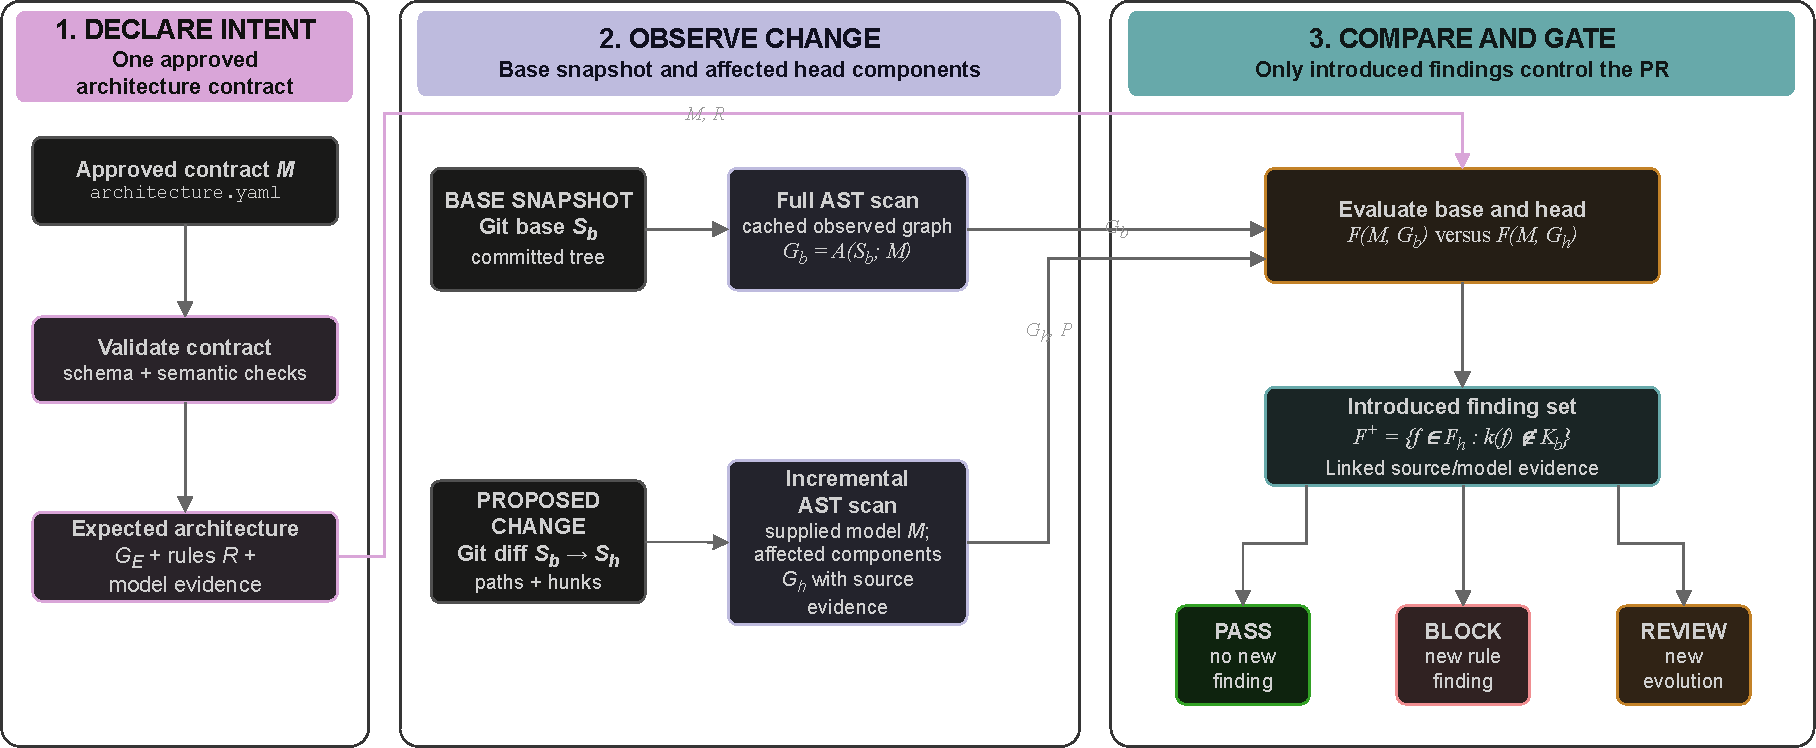
\includegraphics[width=\textwidth]{figures/Fig-1.pdf}
  \caption{ArchSync Phase 3 system architecture. The three-stage pipeline separates approved intent, base/head observation, and the pull-request gate. The model remains authoritative; only findings introduced by the Git diff determine PASS, BLOCK, or REVIEW.}
  \Description{Stage one validates the approved architecture contract into an expected graph, rules, and model evidence. Stage two builds a cached base graph and incrementally reconstructs the proposed head with source evidence. Stage three compares base and head findings, keeps the introduced set, and maps it to PASS, BLOCK, or REVIEW.}
  \label{fig:architecture}
\end{figure*}

The architecture is divided across focused repositories. \archsyncrepository{archsync-core}{https://github.com/Little-Boy-s-ArchSync/archsync-core} contains the architecture contract and deterministic conformance functions. \archsyncrepository{archsync-guardian}{https://github.com/Little-Boy-s-ArchSync/archsync-guardian} contains analyzers and findings. \archsyncrepository{archsync-benchmark}{https://github.com/Little-Boy-s-ArchSync/archsync-benchmark} contains the controlled development benchmark. \archsyncrepository{archsync-examples}{https://github.com/Little-Boy-s-ArchSync/archsync-examples} contains readable models and generated views. \archsyncrepository{archsync-mcp}{https://github.com/Little-Boy-s-ArchSync/archsync-mcp} is reserved for a later interaction layer and is excluded from the initial experiment. The named draft exposes these real repository links; the double-blind build replaces them with blinded artifact labels.

\section{Implementation}

\subsection{Prototype and Detector Logic}

\archsyncrepository{archsync-core}{https://github.com/Little-Boy-s-ArchSync/archsync-core} implements the architecture contract, schema and semantic validation, normalized graph comparison, and deny/allow/require/require-path rules. \archsyncrepository{archsync-guardian}{https://github.com/Little-Boy-s-ArchSync/archsync-guardian} implements TypeScript extraction, source evidence, and the Git-diff gate. Guardian delegates conformance semantics to Core so repository and incremental checks use the same rule engine.

For a concrete PostgreSQL example, consider the following code inside the \texttt{order-service} component:
\begin{verbatim}
import { Pool as PgPool } from "pg";
const db = new PgPool({
  connectionString:
    "postgres://postgres:5432/orders"
});
await db.query("select 1");
\end{verbatim}
The import detector records \texttt{PgPool} as a local name for a recognized \texttt{pg} constructor. The initializer pass recognizes \texttt{new PgPool}, resolves the inline \texttt{connectionString}, and associates \texttt{db} with target \texttt{postgres}, derived from the URL hostname. At \texttt{db.query}, the call detector requires that receiver association before emitting the directed edge $(\texttt{order-service},\texttt{data},\texttt{postgres})$. Merely importing \texttt{pg}, constructing an unrelated client, or calling an unrelated object's \texttt{query} method does not satisfy this detector. Construction alone does not emit the database-access edge. Evidence identifies the query call's file, line, column, detector, and excerpt.

The analysis uses per-file identifier maps and four passes over variable declarations; it is not general alias analysis or interprocedural data-flow analysis. Imported client wrappers, arbitrary reassignment, shadowed identifiers, and relationships requiring resolution across files are not comprehensively handled. Endpoint resolution uses literals, mapped variables, and naming conventions such as \texttt{DATABASE\_URL} for \texttt{postgres}. For binary expressions it tries the right-hand expression first; this deterministic heuristic does not evaluate runtime environment values or branch conditions. The PostgreSQL evidence confidence of 0.99 is a fixed detector annotation, not a calibrated probability. Redis operations similarly require a recognized client, and AMQP operations require a channel associated with a recognized connection.

\subsection{Controlled Evaluation Artifact}

\archsyncrepository{archsync-benchmark}{https://github.com/Little-Boy-s-ArchSync/archsync-benchmark} supplies the synthetic Order Platform, 20 executable patches with group-authored ground truth, and the 40-signal positive/hard-negative corpus. Each patch runs on a fresh copy. Git-diff experiments additionally construct a baseline commit, perform cold and warm checks, and compare incremental head observations with a separate full scan. This full scan checks incremental equivalence; it does not independently establish extraction accuracy.

Measurements use \archsynccommit{Core}{https://github.com/Little-Boy-s-ArchSync/archsync-core}{2affbbb0da859a32b9b9079b4bf718fc7b14993b}{2affbbb0da85}, \archsynccommit{Guardian}{https://github.com/Little-Boy-s-ArchSync/archsync-guardian}{8779bf7965b3bd15f25834f17ca5321c85ae3f43}{8779bf7965b3}, and \archsynccommit{Benchmark}{https://github.com/Little-Boy-s-ArchSync/archsync-benchmark}{24d63ebf2fc3075a1d64f1eaff38cdc0b7f586fb}{24d63ebf2fc3}. Later development heads do not replace these measured artifacts. Source/patch manifests, raw results, package hashes, historical verification commands, and the detector/gate audit remain in the supplementary artifact. These controls support inspection, not independent accuracy evidence. \texttt{archsync-mcp} is excluded.

\section{Controlled Verification Methodology}
\textbf{D1 development benchmark.} An Order Platform baseline has five components and five directed relationships. Twenty isolated patches comprise nine no-impact changes, seven violations, and four evolutions. Cases include service bypass, required-edge removal, allow and require-path rules, PostgreSQL aliases, Redis and AMQP additions, a new service, and non-architectural lookalikes. Each declares changed files, graph delta, classification, rule identifiers, and source evidence. Topology intent originated before analyzer integration, but patches and exact evidence lines were refined alongside it. D1 is a co-developed regression oracle, not a blinded holdout.

\textbf{D2 detector corpus.} Five detector groups (HTTP, PostgreSQL, Redis, AMQP publish, and AMQP consume) each contain four positive and four hard-negative source lines: 40 annotated signals in total. Positives exercise aliases, namespaces, environment fallbacks, and supported operations. Negatives include unused imports, custom functions, method-name collisions, comments, and string literals. An annotation binds detector, file, line, expected edge, and source substring. D2 was authored from known v 0.1 weaknesses and guided v 0.2, so the paired result measures targeted regression behavior.

\textbf{Execution and P3 replay.} D1 validates model, manifest, hashes, and patch applicability, then executes an unchanged baseline twice and each individually patched copy twice: 42 analyzer runs. D2 executes each of two pinned analyzer versions twice. P3 creates a fresh Git baseline for every D1 patch, applies it, and runs one cold and one warm diff check. A separate full-head scan provides an equivalence oracle. The same 20 patches are reused, not counted as a third independent dataset. Normalized duplicate outputs exclude timing and cache state. The functional workflow was reproduced on clean Linux and Windows CI runners; latency comes only from the recorded Windows environment.

\begin{figure*}[t]
\centering
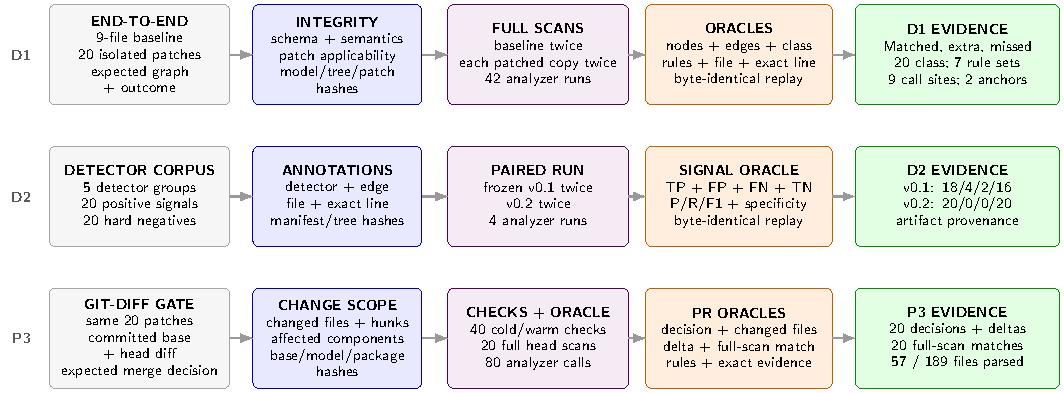
\includegraphics[width=\textwidth]{figures/Fig-2.pdf}
\caption{Controlled verification: full-graph D1 changes, D2 source signals, and incremental P3 replay. All routes use co-developed data.}
\Description{D1 validates isolated patches; D2 checks annotated signals; P3 checks cold and warm Git-diff results against a full scan.}
\label{fig:evaluation-protocol}
\end{figure*}

\textbf{Measures.} D1 reports matched, extra, and missed graph items, separating changed items from repeated baseline structure. Empty changed sets contribute no positive item. Classification uses all 20 cases; rule agreement uses seven violations; evidence agreement splits the original 11 cases post hoc into nine call-site and two missing-relation anchor cases (08 and 17). It requires declared file/line matches per case, not per-finding recall; labels and acceptance rules are unchanged. D2 counts annotated detector signals, not unique edges, with
\[
P=\frac{TP}{TP+FP},\quad R=\frac{TP}{TP+FN},
\]
\[
F_1=\frac{2PR}{P+R},\quad Sp=\frac{TN}{TN+FP}.
\]
Specificity covers only declared hard negatives. P3 checks decision, changed-file and architecture-delta equality, full-scan equivalence, replay, and expected cache miss/hit. Parsed scope is the ratio of affected-component TypeScript file instances to full-head instances. Latency uses nearest-rank $x_{(\lceil pn\rceil)}$ at p50/p95. With 20 samples, p50 is the tenth observation, not the average of the middle pair. Original timings are descriptive, not population or comparative-performance estimates. Node 22.16.0, Windows 10.0.26200, i7-13650HX and 20 logical CPUs were recorded. RAM, power mode, background/thermal load and filesystem-cache state were not recorded.

\textbf{Engineering gates.} The existing protocol required D1 precision/recall at least 0.85, exact decisions/rules/evidence, and deterministic replay; D2 required all annotated positives and negatives correct; P3 required exact replay/full-scan agreement and cache behavior. These are development acceptance rules, not statistical standards. The paper reports counts even where its underlying engineering gate computes rates.

\textbf{Proposed external comparison.} External comparison remains future work; no external-tool comparison was executed within the reported evaluation; no accepted comparator result or common label mapping is available. A module-dependency analyzer is a candidate, but module imports and typed service calls need an explicit, independently reviewed mapping before comparative scoring. The proposed protocol must freeze repositories, versions, configurations, dependency-resolution conditions, and independently authored ground truth before inspecting outputs. Unsupported relations must be separated from misses within common supported scope. The protocol rejects a comparator without a non-empty semantic intersection and requires separately freezing any adapter. A capability discussion cannot complete the baseline or supply an accuracy estimate. Reusing D1 would remain a development-set comparison rather than an independent holdout.

\section{Controlled Verification Results}

\begin{table}[t]
  \caption{D1 counts on 20 co-developed patches. The five changed nodes and 12 changed edges are regression items, not independent samples of general accuracy; full-graph counts repeat baseline structure.}
  \label{tab:detection-results}
  \centering
  \small
  \begin{tabular}{lrrr}
    \hline
    Measure & Matched & Extra & Missed \\
    \hline
    Full-graph nodes & 105 & 0 & 0 \\
    Full-graph edges & 108 & 0 & 0 \\
    Changed nodes & 5 & 0 & 0 \\
    Changed edges & 12 & 0 & 0 \\
    \hline
  \end{tabular}
\end{table}

\begin{table}[t]
  \caption{Decision, evidence, and replay outcomes on controlled D1 cases.}
  \label{tab:outcome-results}
  \centering
  \small
  \begin{tabular}{lrr}
    \hline
    Measure & Matches & Total \\
    \hline
    Classification & 20 & 20 \\
    Violation rule set & 7 & 7 \\
    Call-site file and line & 9 & 9 \\
    Missing-relation anchor file and line & 2 & 2 \\
    Deterministic cases & 20 & 20 \\
    \hline
  \end{tabular}
\end{table}

\begin{table}[t]
  \caption{P3 Git-diff gate outcomes and measured scope on the D1 replay.}
  \label{tab:phase3-results}
  \centering
  \small
  \begin{tabular}{lr}
    \hline
    Measure & Result \\
    \hline
    Classification agreement & 20/20 \\
    Merge-decision agreement & 20/20 \\
    Changed-file agreement & 20/20 \\
    Architecture-delta agreement & 20/20 \\
    Incremental/full-scan agreement & 20/20 \\
    Violation rule-set agreement & 7/7 \\
    Call-site exact line & 9/9 \\
    Anchor exact line & 2/2 \\
    Cache hit on repeated check & 20/20 \\
    Normalized cold/warm replay & 20/20 \\
    Incremental files / head files & 57/189 \\
    Cold p50 / p95 (ms) & 518.51 / 531.05 \\
    Warm p50 / p95 (ms) & 242.62 / 249.30 \\
    \hline
  \end{tabular}
\end{table}

\begin{table*}[t]
  \caption{D2 within-tool regression confusion matrices for the frozen v0.1 and provenance-aware v0.2 analyzers on the same co-developed 40-signal corpus.}
  \label{tab:pattern-results}
  \centering
  \small
  \begin{tabular}{lrrrrrrrr}
    \hline
    & \multicolumn{4}{c}{v0.1} & \multicolumn{4}{c}{v0.2} \\
    Detector & TP & FP & FN & TN & TP & FP & FN & TN \\
    \hline
    \texttt{fetch} & 4 & 0 & 0 & 4 & 4 & 0 & 0 & 4 \\
    PostgreSQL & 4 & 1 & 0 & 3 & 4 & 0 & 0 & 4 \\
    Redis & 2 & 0 & 2 & 4 & 4 & 0 & 0 & 4 \\
    AMQP publish & 4 & 2 & 0 & 2 & 4 & 0 & 0 & 4 \\
    AMQP consume & 4 & 1 & 0 & 3 & 4 & 0 & 0 & 4 \\
    \hline
    Overall & 18 & 4 & 2 & 16 & 20 & 0 & 0 & 20 \\
    \hline
  \end{tabular}
\end{table*}

\textbf{RQ1: graph reconstruction and detector signals.}
The unchanged repository was reconstructed as five components and five relationships with a no-impact classification. Table~\ref{tab:detection-results} reports no false positive or false negative in D1. Full-graph totals aggregate 105 expected nodes and 108 expected edges across 20 patched repositories. Only five node changes and 12 edge changes contribute positive changed-graph items. These finite, co-developed cases test contract agreement; they do not estimate performance on unseen projects.

Table~\ref{tab:pattern-results} gives the signal-level regression result. On D2, v0.1 achieved precision 0.818, recall 0.900, F1 0.857, and specificity 0.800. Its four false positives were a PostgreSQL-shaped local query, two AMQP-publish lookalikes, and an AMQP-consume lookalike; its two false negatives were Redis \texttt{hSet} and \texttt{lPush}. On the same annotated signals, v0.2 matched all 20 positives and rejected all 20 annotated negatives (precision, recall, F1, and specificity each 1.000 on this corpus). Package-provenance tracking removed the four method-name false positives, while the expanded Redis operation set recovered the two missed positives. Because D2 was constructed from known v0.1 weaknesses, this is targeted regression evidence and not an estimate over arbitrary TypeScript syntax or an external baseline comparison.

\textbf{RQ2: change classification.}
ArchSync matched all 20 D1 labels: nine no-impact, seven violation, and four evolution cases. It also matched the complete expected rule-identifier set for all seven violations. The added allow and require-path cases exercise rule semantics beyond direct deny and require checks. Redis, AMQP, Fraud Service, and payment-cache additions were classified as evolution rather than violation, preserving a human-review path.

\textbf{RQ3: evidence localization.}
All 11 finding-bearing D1 cases are split post hoc into call-site file/line agreement in 9/9 cases and anchor agreement in 2/2 cases, for missing-edge case 08 and missing-path case 17. Both P2 and P3 satisfy the separate checks. These are case-level outcomes: case 15 has two violated rules but contributes one case. An anchor is not a localized absent call, and neither measure evaluates ranking, all supporting locations, or reviewer effort.

\textbf{RQ4: determinism and reproducibility.}
The D1 baseline and all 20 cases produced byte-identical normalized JSON across duplicate executions, giving 42 current-version executions with no replay mismatch. Both D2 analyzer versions were also deterministic across their duplicate runs. P3 produced identical normalized cold and warm results for 20/20 cases, matched all 20 declared architecture deltas, matched a separate full head scan in all 20 cases, and hit the baseline cache on every repeated check. As Table~\ref{tab:phase3-results} shows, component-incremental analysis parsed 57 of 189 TypeScript file instances, $r_{\mathrm{parse}}=0.3016$. On the recorded Windows environment, warm nearest-rank p50 latency was 242.62 ms compared with 518.51 ms cold, a descriptive 53.2\% reduction; warm p95 was 249.30 ms compared with 531.05 ms cold. Local verification reproduced all stored results and repository gates. GitHub Actions independently reproduced the functional benchmark, detector, and Git-diff evidence on both \texttt{ubuntu-latest} and \texttt{windows-latest}; timing values were not treated as cross-platform acceptance thresholds.

\textbf{Boundary of the reported evidence.}
The observations above come from D1, D2, and the P3 reuse of D1. No external-tool result is accepted into this evaluation, and no common label mapping has been established for comparative scoring. The internal v0.1--v0.2 detector comparison and incremental/full-scan equivalence therefore answer different questions from an external baseline: the former exposes targeted regression behavior, while the latter checks whether scoped execution preserves this implementation's full-scan result.

Exact agreement with these oracles does not establish that the expected architecture is complete or appropriate for another system. In particular, a missed relationship outside the detector vocabulary can be absent from both incremental and full scans without producing an equivalence mismatch. Similarly, duplicate executions can reproduce the same incorrect inference. The graph, evidence-location, decision, and replay checks are complementary consistency checks; they do not substitute for independently authored semantic labels or a separately evaluated tool.

\section{Discussion}
The results establish agreement between implemented contracts and their development oracles. D2 shows why end-to-end graph counts alone are insufficient: repeated baseline structure can dominate totals, while hard-negative source locations expose method-name collisions. Its six corrected v 0.1 errors support targeted diagnosis and regression protection, not an unbiased estimate of improvement on unseen programs.

The three-way decision separates forbidden relationships from changes requiring a design decision. P3 reports historical findings while gating only introduced findings, permitting gradual adoption without treating historical keys as new findings. REVIEW neither approves evolution nor rewrites the expected model. The evaluated implementation has no durable rejection disposition: rejecting an evolution requires changing or withdrawing the proposed code and rerunning the check; unchanged inputs still yield REVIEW. Accepting it requires a separately reviewed model change. Owner protection is therefore an organizational prerequisite, not an experimentally validated property of the gate.

Component scoping parsed 57/189 file instances and warm caching reduced the recorded nearest-rank p50 from 518.51 to 242.62ms. Those observations combine parsing, Git processes, cache I/O, comparison, and reporting; they do not isolate algorithmic cost or establish scale. Next experiments require independently annotated real repositories and histories, capability-aligned external baselines, and a practitioner pilot measuring false-block burden, review effort, and model-change governance. IaC, runtime, AI assistance, and other language analyzers remain unevaluated extensions.

\section{Threats to Validity}
\textbf{Construct validity.} Typed topology and explicit rules do not measure responsibility, rationale, runtime quality, or developer usefulness. Evidence agreement requires one matching location, not complete or well-ranked evidence. An absent relationship has only a deterministic component anchor. D2 signals can share an edge, and its negatives do not represent all unsupported syntax. Parsed-file counts measure analysis scope, not CPU work.

\textbf{Internal validity.} The authors developed the analyzer and both datasets. D1 topology intent preceded integration, but patch implementations and exact evidence lines co-evolved with the analyzer. D2 targeted known v0.1 errors and guided v0.2. Replaying D1 in P3 adds incremental checks, not independent observations. Hashes, raw predictions, mutation checks, and duplicate execution expose inconsistency but do not establish independent ground truth.

\textbf{External and conclusion validity.} One small synthetic system, 20 patches, and 40 curated signals cannot estimate general TypeScript accuracy. The five changed nodes, 12 changed edges, seven violation rule sets, and 11 evidence cases are finite regression items. Wrappers, dynamic endpoints, dependency injection, generated code, unconventional repositories, other languages, and runtime-only relationships remain outside evaluated coverage. Latency is descriptive from one environment; there is no workload-population inference, scalability study, or significance test. No industrial deployment or developer study was executed. Later repository protection is not experimental evidence of a non-bypassable human-governed workflow.

\textbf{Comparative validity.} The external comparison remains proposed and contributes no reported execution or result. No accepted common label mapping exists. Differences between import and service-call semantics require a reviewed scoring abstraction. Independently authored data and capability-matched ground truth remain necessary. Duplicate replay can reproduce an incorrect inference, and incremental/full-scan agreement can preserve omissions shared by both modes. These consistency checks cannot establish semantic completeness.

\textbf{Literature positioning.} The narrative review carries source-selection and interpretation bias and may omit approaches. Coverage completeness and absence-of-evidence claims are outside its design, not deferred SLR deliverables. Related studies can share projects or implementations, so citation breadth does not imply independent replication.

\textbf{Reliability.} Pinned artifacts, normalized ordering, isolated patches, duplicate execution, and clean Linux/Windows functional checks support reproducibility. The frozen v0.1 result is provenance-validated rather than continuously regenerated; Windows timing is not a cross-platform performance claim. These controls address repeatability of the controlled experiment, not the independence of its labels.

\section{Conclusion and Future Work}

ArchSync implements a deterministic bridge between a declared architecture contract and a source-derived TypeScript service graph. On the co-developed development datasets, its graph, classification, evidence-location, replay, and incremental/full-scan outputs agree with the declared regression oracles. The targeted detector corpus also exposes concrete errors in the earlier analyzer and verifies that provenance tracking addresses those cases.

They do not establish general accuracy, comparative advantage, or governance effectiveness: the datasets co-evolved with the implementation, no accepted external comparison or common label mapping is available, and no independent real-world holdout exists. The analyzer never rewrites the model; evolution needs human review. Next studies require an independent multi-repository holdout, capability-matched external comparison and real pull-request pilot. Only after those gates produce auditable evidence should claims extend to external accuracy, performance or developer value.

\ifarchsyncanonymous\else
\noindent\begin{minipage}{\columnwidth}
\section*{Author Information and Contributions}

\noindent\textbf{Vo Duc Hieu} (ORCID: \href{https://orcid.org/0009-0007-5389-5177}{0009-0007-5389-5177}) - Conceptualization; Methodology; Software; Project administration; Writing.

\noindent\textbf{Tran Minh Hoang} (ORCID: \href{https://orcid.org/0009-0000-0302-1841}{0009-0000-0302-1841}) - Software; AI methodology; Validation.

\noindent\textbf{Ha Hoang Bach} (ORCID: \href{https://orcid.org/0009-0000-5118-0660}{0009-0000-5118-0660}) - Investigation; Data curation; Formal analysis; Evaluation.

\noindent\textbf{Le Van Kiet} (ORCID: \href{https://orcid.org/0009-0007-8434-882X}{0009-0007-8434-882X}) - Software; Validation; Reproducibility.

\noindent\textbf{Hoang Nguyen The} - Supervision; Methodology; Writing - review and editing.

\noindent\textbf{Minh Tam Phan} - Supervision; Methodology; Writing - review and editing.
\end{minipage}
\fi
% Balance the reference continuation without changing IEEE fonts or margins.
\IEEEtriggeratref{18}


\bibliographystyle{archsync-ieee}
\bibliography{references}

\end{document}
